\documentclass[UTF8,a4paper,12pt]{ctexart}

\usepackage{geometry}
\usepackage{graphicx}
\usepackage{booktabs}
\usepackage{longtable}
\usepackage{array}
\usepackage{float}
\usepackage{xcolor}
\usepackage{listings}
\usepackage{enumitem}
\usepackage{hyperref}
\usepackage{caption}

\geometry{left=2.5cm,right=2.5cm,top=2.5cm,bottom=2.5cm}
\graphicspath{{figures/}{./}}

\hypersetup{colorlinks=true,linkcolor=blue,urlcolor=blue,citecolor=blue}

\lstset{
    basicstyle=\ttfamily\small,
    breaklines=true,
    frame=single,
    backgroundcolor=\color{gray!8},
    keywordstyle=\color{blue},
    commentstyle=\color{gray},
    stringstyle=\color{teal},
    columns=fullflexible
}

\title{成员 F：PreLog 论文复现、Online-Boutique 迁移实验与 AIOps Agent 封装报告}
\author{成员 F}
\date{\today}

\begin{document}

\maketitle

\begin{abstract}
本报告整理成员 F 在软件测试与维护课程大作业中的工作，包括 SIGMOD 2024 PreLog 论文复现、Online-Boutique 日志与指标数据上的迁移实验、Metric-Event Baseline 辅助验证，以及轻量级 AIOps Agent 的封装实现。实验首先在官方 BGL 日志数据集上复现 PreLog，证明论文方法和代码流程能够成功运行；随后将模型迁移到本组 Online-Boutique 数据，但观察到明显的单类别退化现象。为验证组内数据本身是否包含有效异常信号，进一步将 Prometheus/Grafana CSV 指标转化为 Metric-Event 日志，并使用 TF-IDF + Logistic Regression 进行对照实验，取得较高识别效果。最后实现一个 AIOps Agent，监听成员 E 的异常检测结果 CSV，并自动完成异常触发、根因解释和 Kubernetes 修复命令生成，形成“检测--诊断--处置”的智能运维闭环。
\end{abstract}

\tableofcontents
\newpage

\section{任务背景与成员 F 工作范围}

本课程大作业围绕微服务系统的部署、测试、故障注入、异常检测与智能运维展开。组内系统最终选用 Online-Boutique 作为微服务实验对象。成员 F 的主要任务包括：

\begin{enumerate}[label=\arabic*.]
    \item 选择并复现一篇日志异常检测论文，本报告选择 SIGMOD 2024 PreLog；
    \item 将论文算法尝试迁移到本组 Online-Boutique 实验数据；
    \item 对 Online-Boutique 日志与指标数据进行处理、实验与可视化；
    \item 封装一个轻量级 AIOps Agent，接收异常检测结果并输出诊断解释和修复建议。
\end{enumerate}

整体工作流程如下：

\begin{center}
\begin{tabular}{p{3cm}p{10cm}}
\toprule
阶段 & 工作内容 \\
\midrule
论文复现 & 配置 PreLog 环境，在 BGL 数据集上跑通训练与评估流程 \\
组内数据迁移 & 收集 Online-Boutique 日志、Prometheus CSV 指标，转化为 PreLog 输入格式 \\
结果分析 & 分析 PreLog 在组内数据上的退化现象，并用 Metric-Event Baseline 验证数据可分性 \\
Agent 封装 & 监听成员 E 的算法结果，生成根因解释和 kubectl 修复命令 \\
\bottomrule
\end{tabular}
\end{center}

\section{PreLog 论文与复现目标}

\subsection{论文方法概述}

PreLog 是一种面向日志任务的预训练与下游适配方法。其核心思想是先利用大规模日志语料学习日志文本中的语义与模式，再通过分类任务完成异常检测。对于日志异常检测任务，输入为日志文本，输出为类别标签，例如：

\begin{itemize}
    \item \texttt{clean normal}：正常日志；
    \item \texttt{faulty}：异常日志。
\end{itemize}

在工程实现上，PreLog 使用 prompt template 和 verbalizer 将日志分类问题转换为语言模型可处理的任务。成员 F 的复现目标是：

\begin{enumerate}[label=\arabic*.]
    \item 跑通官方 PreLog 代码与环境；
    \item 在官方 BGL 数据集上得到可接受复现结果；
    \item 尝试将 PreLog 迁移到本组 Online-Boutique 数据；
    \item 分析迁移效果和局限。
\end{enumerate}

\subsection{复现环境}

实验环境如下：

\begin{itemize}
    \item 操作系统：Windows + WSL Ubuntu；
    \item Python 环境：Miniconda，Python 3.8；
    \item 主要依赖：PyTorch、Transformers、Accelerate、scikit-learn、pandas、matplotlib；
    \item GPU：CUDA 可用环境；
    \item 微服务系统：Online-Boutique；
    \item 故障注入：ChaosMesh。
\end{itemize}

\section{PreLog 官方数据集复现}

\subsection{BGL 数据集实验}

首先在官方 BGL 数据集上运行 PreLog，验证论文代码和训练流程是否可复现。实验命令核心参数如下：

\begin{lstlisting}[language=bash]
CUDA_VISIBLE_DEVICES=0 accelerate launch --mixed_precision fp16 train.py \
  --dataset BGL \
  --model-path /mnt/e/software_test_project/prelog_data/PreLog \
  --train-file /mnt/e/software_test_project/prelog_data/BGL/train/1.json \
  --test-file /mnt/e/software_test_project/prelog_data/BGL/test.json \
  --prompt-template prompt_template.txt \
  --verbalizer anomaly_detection/verbalizer.txt \
  --batch-size 2 \
  --lr 3e-5 \
  --max-length 512 \
  --do-train \
  --do-eval
\end{lstlisting}

\subsection{BGL 复现结果}

在 BGL 数据集上，PreLog 能够正常完成训练和评估，得到如下结果：

\begin{center}
\begin{tabular}{lcccc}
\toprule
类别 & Precision & Recall & F1-score & Support \\
\midrule
clean normal & 0.999 & 0.998 & 0.994 & 215418 \\
faulty & 0.886 & 0.990 & 0.935 & 20257 \\
accuracy & \multicolumn{3}{c}{0.988} & 235675 \\
macro avg & 0.943 & 0.989 & 0.964 & 235675 \\
weighted avg & 0.989 & 0.988 & 0.989 & 235675 \\
\bottomrule
\end{tabular}
\end{center}

其中，异常类 \texttt{faulty} 的 F1-score 达到 0.935，说明 PreLog 的官方实验流程已成功复现。该结果作为本成员论文复现部分的核心结果。

\begin{figure}[H]
    \centering
    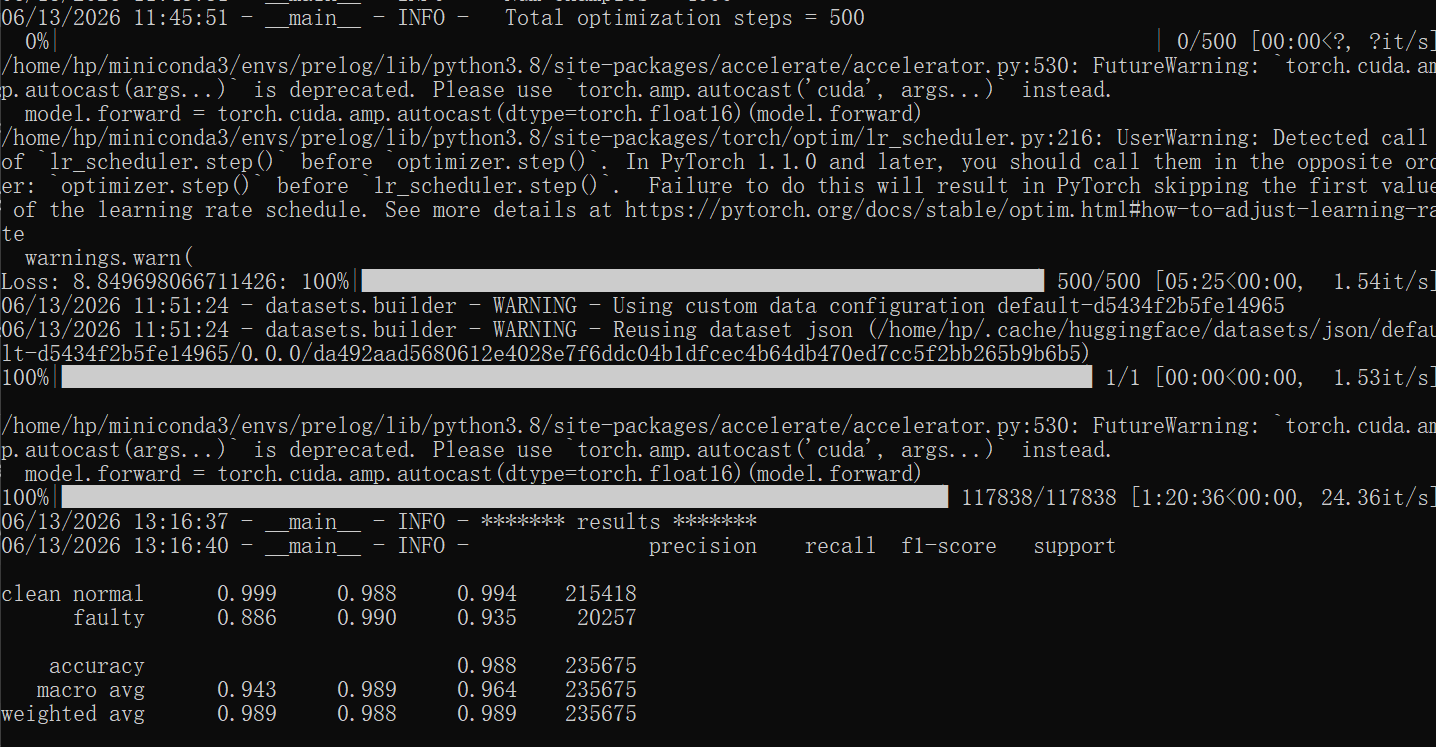
\includegraphics[width=0.95\linewidth]{PreLog_BGL_result.png}
    \caption{PreLog 在 BGL 数据集上的复现结果截图。若没有该图片，可替换为对应终端截图。}
\end{figure}

\section{Online-Boutique 数据处理与迁移实验}

\subsection{组内 Online-Boutique 实验数据}

组内最终选用 Online-Boutique 微服务系统，并设计了三类故障：

\begin{enumerate}[label=\arabic*.]
    \item \textbf{frontend 网络延迟}：导致请求延迟升高；
    \item \textbf{checkoutservice CPU 过载}：导致接口处理缓慢，CPU 和响应时间指标上升；
    \item \textbf{cartservice Pod Kill}：导致服务瞬时不可用和请求失败。
\end{enumerate}

可用数据包括：

\begin{itemize}
    \item Online-Boutique 三个服务日志：\texttt{frontend\_logs.txt}、\texttt{checkoutservice\_logs.txt}、\texttt{cartservice\_logs.txt}；
    \item 新实验 Prometheus/Grafana CSV：\texttt{metrics.csv}；
    \item 旧实验 Prometheus/Grafana CSV：\texttt{metrics\_old.csv}。
\end{itemize}

\subsection{原始日志转 PreLog 输入}

首先尝试将应用日志转化为 PreLog 支持的 JSON 格式，每条样本包含两个字段：

\begin{lstlisting}[language=json]
{"text": "... log text ...", "labels": "clean normal"}
{"text": "... log text ...", "labels": "faulty"}
\end{lstlisting}

标签根据故障注入时间窗口生成：

\begin{itemize}
    \item 新实验故障时间约为：16:24--16:26、16:36--16:40、16:41--16:43；
    \item 非故障窗口标注为 \texttt{clean normal}；
    \item 故障窗口标注为 \texttt{faulty}。
\end{itemize}

\subsection{PreLog 迁移实验结果}

将 PreLog 直接迁移到 Online-Boutique 数据后，模型出现明显单类别退化现象。典型结果如下：

\begin{center}
\begin{tabular}{lcccc}
\toprule
类别 & Precision & Recall & F1-score & Support \\
\midrule
clean normal & 0.000 & 0.000 & 0.000 & 360 \\
faulty & 0.471 & 1.000 & 0.640 & 320 \\
accuracy & \multicolumn{3}{c}{0.471} & 680 \\
macro avg & 0.235 & 0.500 & 0.320 & 680 \\
weighted avg & 0.221 & 0.471 & 0.301 & 680 \\
\bottomrule
\end{tabular}
\end{center}

该结果说明模型几乎将所有样本预测为 \texttt{faulty}，导致 \texttt{faulty} recall 虽然达到 1.000，但 \texttt{clean normal} recall 为 0.000。这不是有效异常检测结果，而是迁移失败或分类边界不稳定的表现。

\begin{figure}[H]
    \centering
    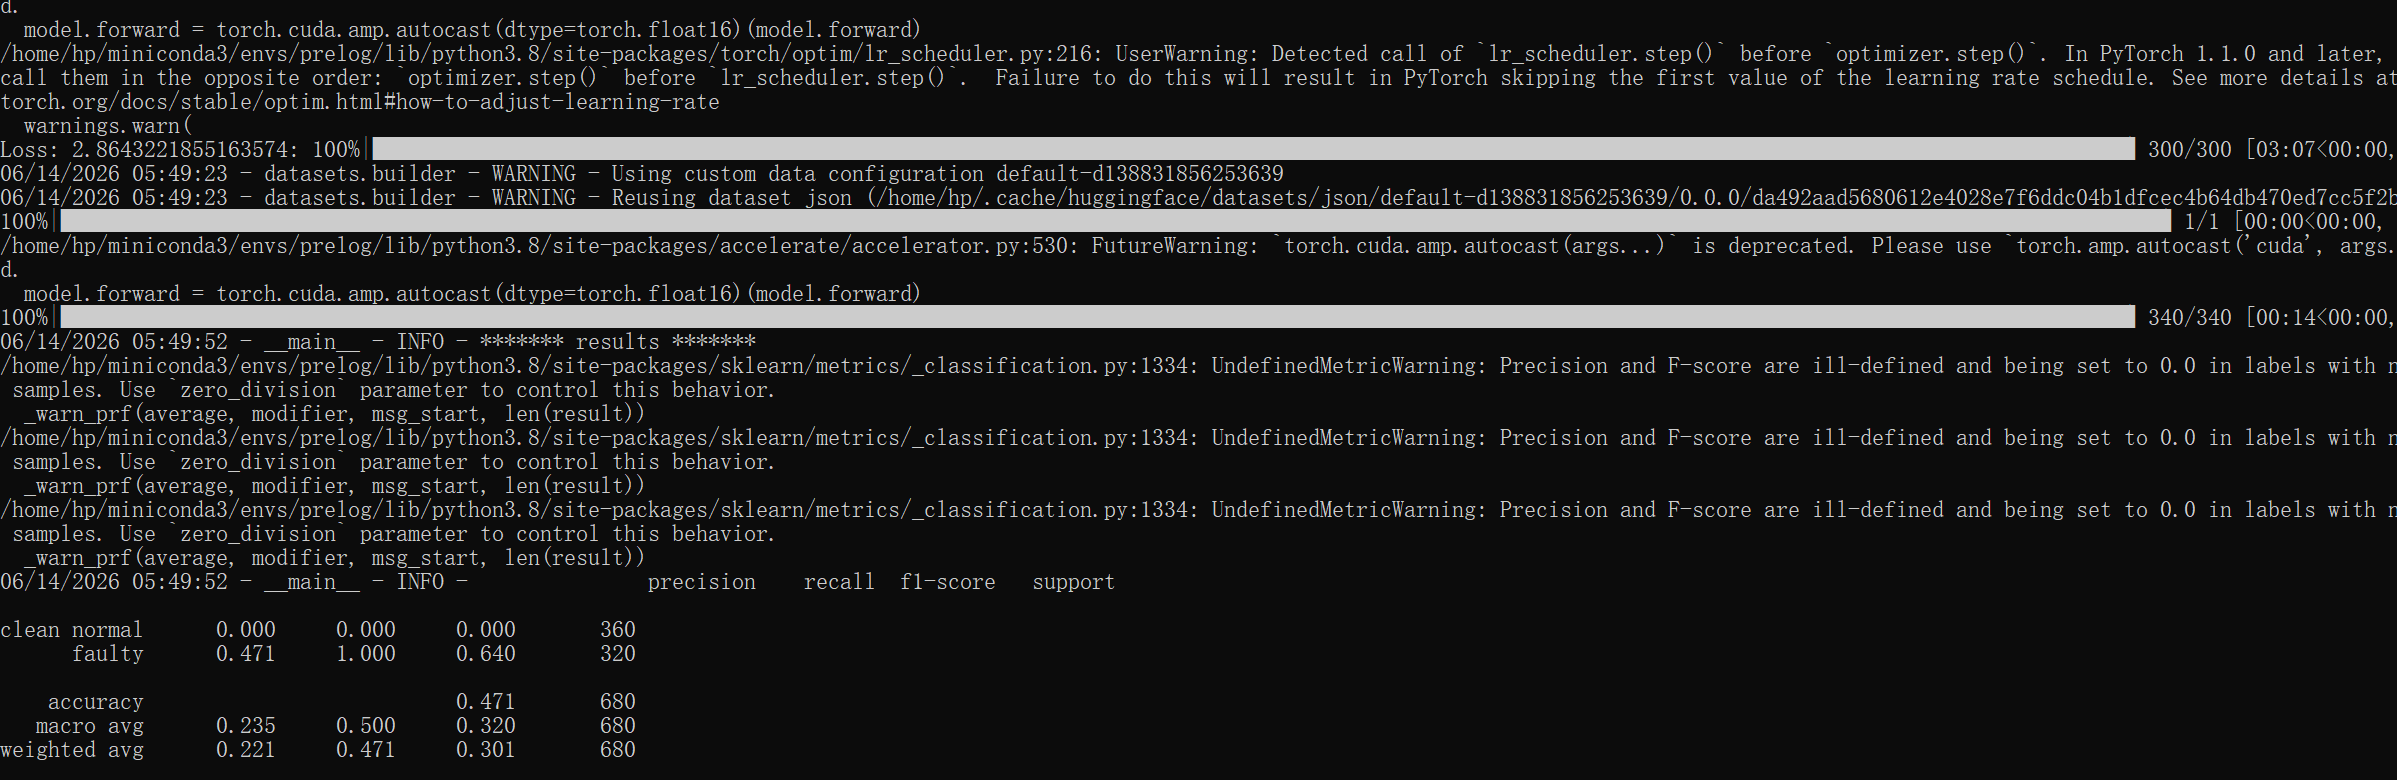
\includegraphics[width=0.95\linewidth]{PreLog_OnlineBoutique_degradation.png}
    \caption{PreLog 在 Online-Boutique 数据上的单类别退化现象。该图建议使用 PreLog 结果截图，而不是 baseline 结果截图。}
\end{figure}

\subsection{退化原因分析}

PreLog 在 BGL 上表现较好，但在 Online-Boutique 上出现单类别退化，主要原因包括：

\begin{enumerate}[label=\arabic*.]
    \item \textbf{数据分布差异明显}：BGL 是典型系统日志，而 Online-Boutique 是业务微服务日志，两者文本模式差异较大；
    \item \textbf{故障信号主要体现在指标层}：网络延迟、CPU 过载等故障不一定在应用日志中产生显式 error 文本；
    \item \textbf{组内数据规模较小}：虽然后来通过连续窗口扩充了样本，但与官方数据集相比仍然较小；
    \item \textbf{模型迁移不稳定}：在不同阈值和类别权重下，模型容易在全 normal 与全 faulty 之间跳变。
\end{enumerate}

因此，本实验不将 PreLog 在 Online-Boutique 上的结果作为有效检测性能，而将其作为“论文模型在组内小规模微服务数据上迁移存在局限”的分析结果。

\section{Metric-Event Baseline 辅助验证}

\subsection{构造 Metric-Event 日志的动机}

由于 Online-Boutique 的故障主要体现在 Prometheus 指标层，因此进一步将 CSV 指标转化为结构化事件日志。每个时间窗口被转化为类似如下的文本：

\begin{lstlisting}
metric_event_log system_online_boutique
ctx0_service_checkoutservice ctx0_z_extreme
ctx0_spike_checkoutservice ctx0_surge_checkoutservice
ctx0_trend_flat
\end{lstlisting}

其中：

\begin{itemize}
    \item \texttt{service\_checkoutservice} 表示相关服务；
    \item \texttt{z\_extreme} 表示该指标相对于正常基线出现极端异常；
    \item \texttt{spike} 和 \texttt{surge} 表示指标尖峰或突增；
    \item \texttt{ctx-1}、\texttt{ctx0}、\texttt{ctx1} 表示前一窗口、当前窗口、后一窗口。
\end{itemize}

该处理本质上是将数值指标转化为文本事件，使其能够被日志类模型或文本分类模型处理。

\subsection{数据集规模}

基于新旧两份 CSV，并按照连续时间窗口进行扩充，最终得到：

\begin{center}
\begin{tabular}{lccc}
\toprule
数据集 & clean normal & faulty & 总计 \\
\midrule
训练集 & 840 & 840 & 1680 \\
测试集 & 360 & 320 & 680 \\
\bottomrule
\end{tabular}
\end{center}

\subsection{Baseline 方法}

为了验证 Metric-Event 日志本身是否包含有效异常信号，使用 TF-IDF + Logistic Regression 进行辅助验证：

\begin{lstlisting}[language=Python]
vectorizer = TfidfVectorizer(
    token_pattern=r"(?u)\b[\w\-]+\b",
    ngram_range=(1, 2),
    min_df=1,
    max_df=0.95,
    sublinear_tf=True,
)

clf = LogisticRegression(
    max_iter=3000,
    class_weight="balanced",
    random_state=42,
    solver="liblinear",
)
\end{lstlisting}

该 baseline 不是 PreLog 论文复现结果，而是用于验证组内指标事件数据是否具有可学习的异常信号。

\subsection{Baseline 实验结果}

Metric-Event Baseline 结果如下：

\begin{center}
\begin{tabular}{lcccc}
\toprule
类别 & Precision & Recall & F1-score & Support \\
\midrule
clean normal & 1.000 & 0.997 & 0.999 & 360 \\
faulty & 0.997 & 1.000 & 0.998 & 320 \\
accuracy & \multicolumn{3}{c}{0.999} & 680 \\
macro avg & 0.998 & 0.999 & 0.999 & 680 \\
weighted avg & 0.999 & 0.999 & 0.999 & 680 \\
\bottomrule
\end{tabular}
\end{center}

混淆矩阵为：

\begin{center}
\begin{tabular}{lcc}
\toprule
真实类别 & 预测 clean normal & 预测 faulty \\
\midrule
clean normal & 359 & 1 \\
faulty & 0 & 320 \\
\bottomrule
\end{tabular}
\end{center}

可见，测试集中只有 1 条 normal 被误报为 faulty，所有 faulty 样本均被识别出来。

\section{结果可视化}

\subsection{Ground Truth 时间线}

\begin{figure}[H]
    \centering
    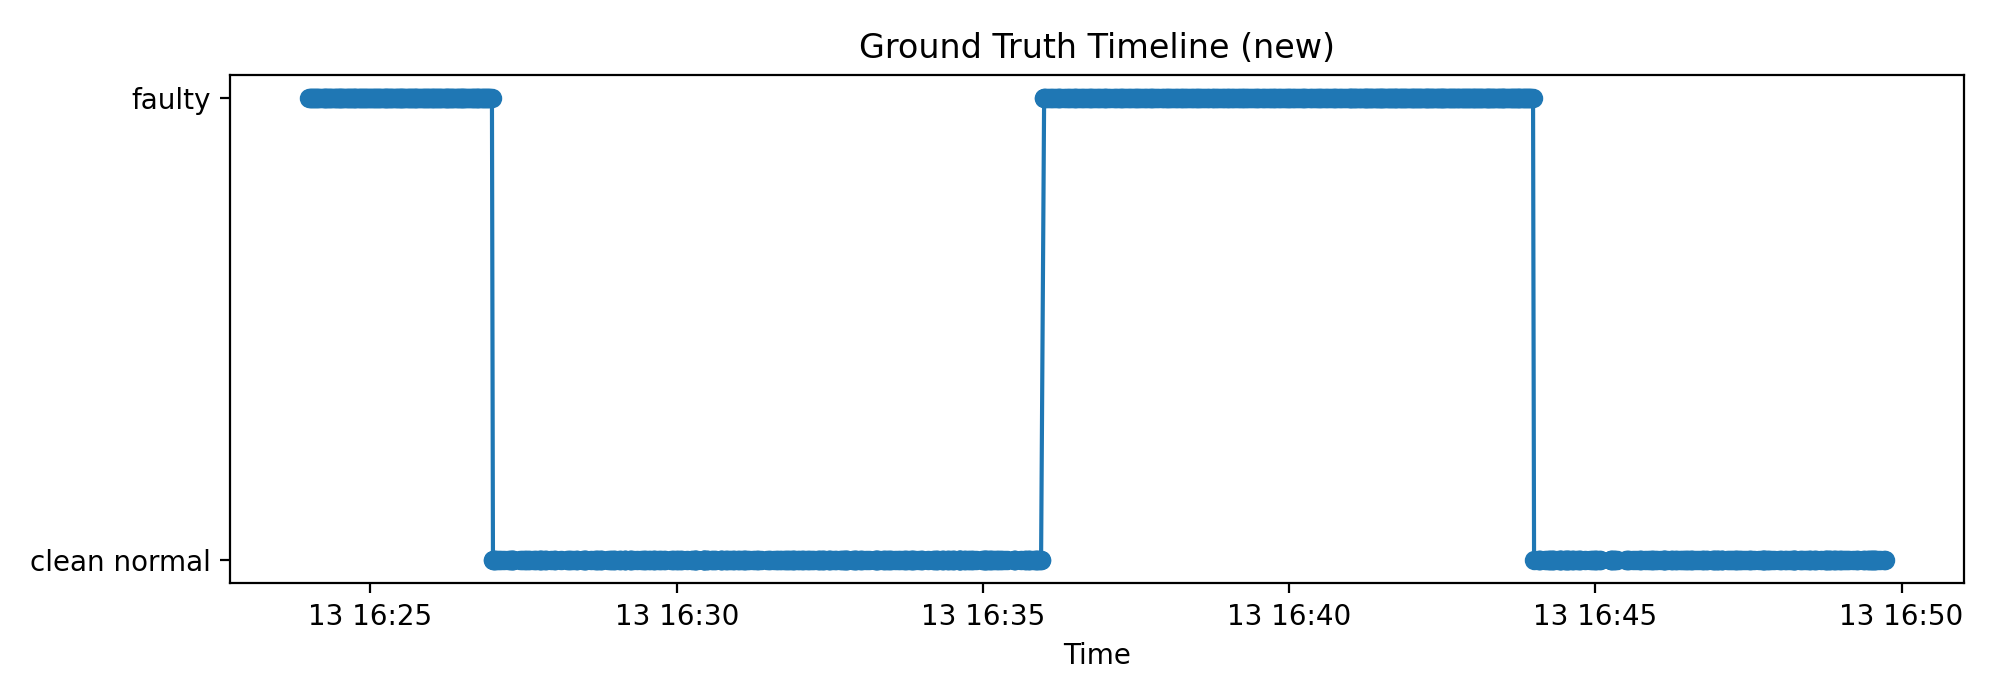
\includegraphics[width=0.95\linewidth]{08_ground_truth_timeline_new.png}
    \caption{新实验数据的 ground truth 时间线。faulty 区间对应故障注入阶段，clean normal 区间对应系统恢复或正常运行阶段。}
\end{figure}

\subsection{混淆矩阵}

\begin{figure}[H]
    \centering
    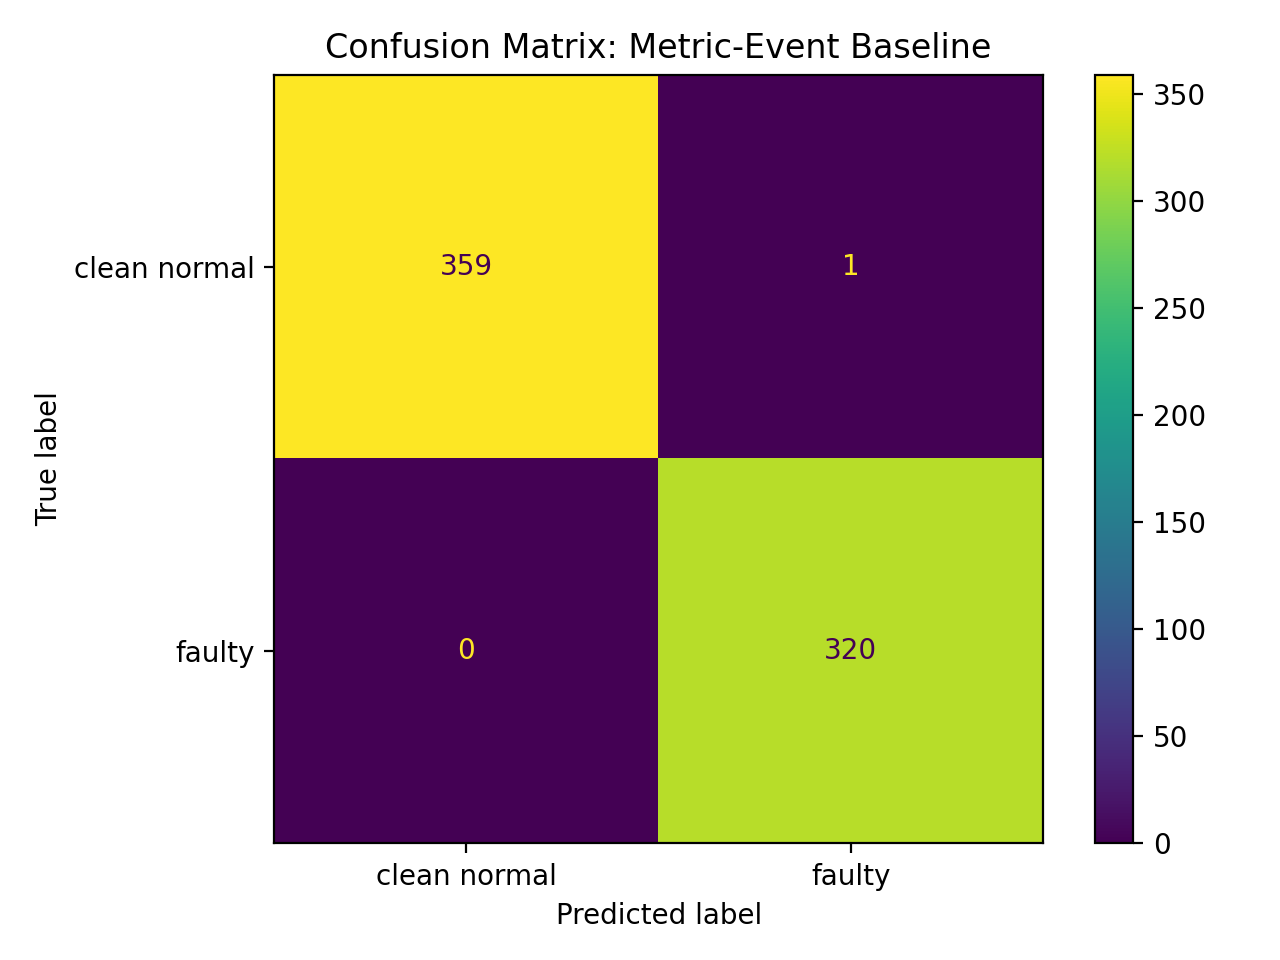
\includegraphics[width=0.75\linewidth]{02_confusion_matrix.png}
    \caption{Metric-Event Baseline 混淆矩阵。测试集共 680 条样本，仅 1 条正常样本被误报为异常。}
\end{figure}

\subsection{Precision、Recall 与 F1-score}

\begin{figure}[H]
    \centering
    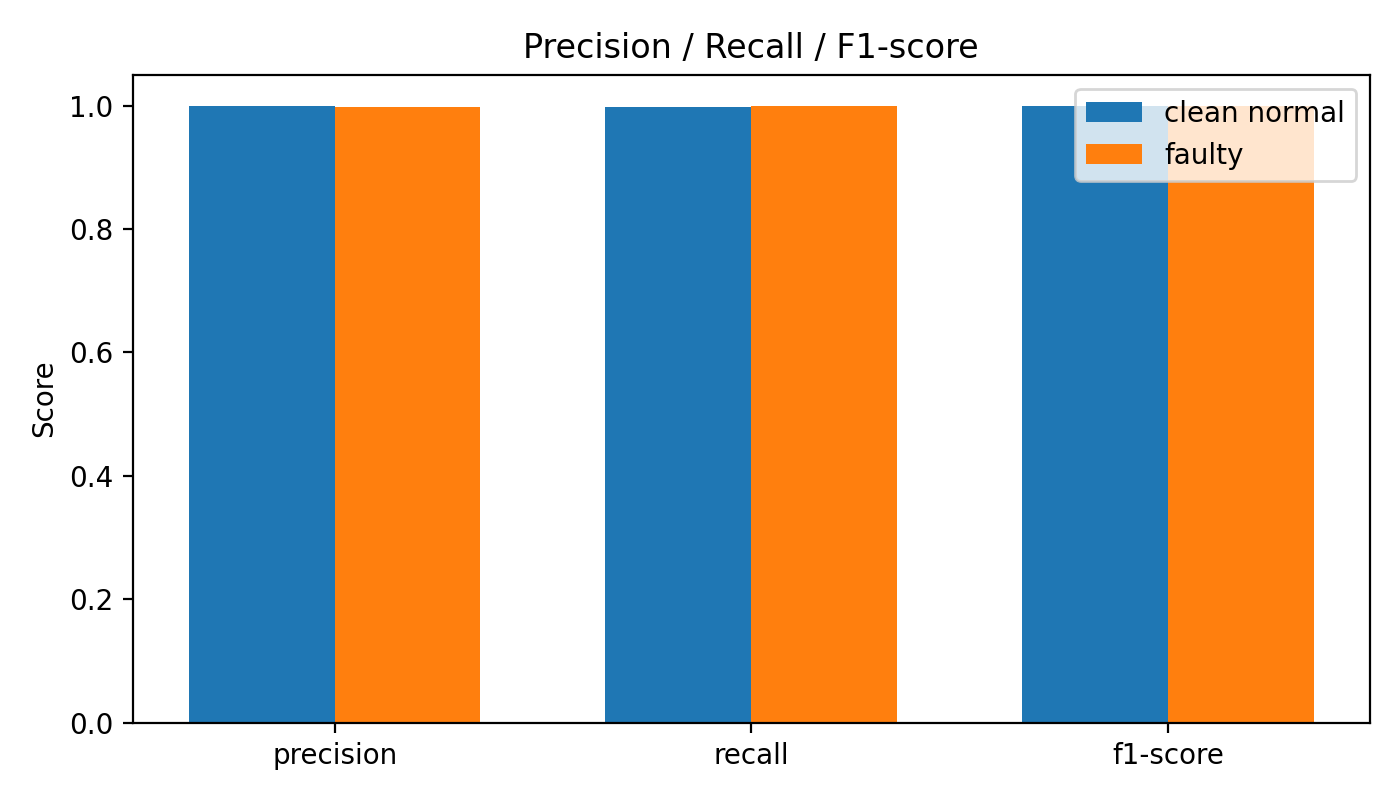
\includegraphics[width=0.80\linewidth]{03_metrics_bar.png}
    \caption{Metric-Event Baseline 的 precision、recall 和 F1-score。两类指标均接近 1。}
\end{figure}

\subsection{Faulty Probability 分布}

\begin{figure}[H]
    \centering
    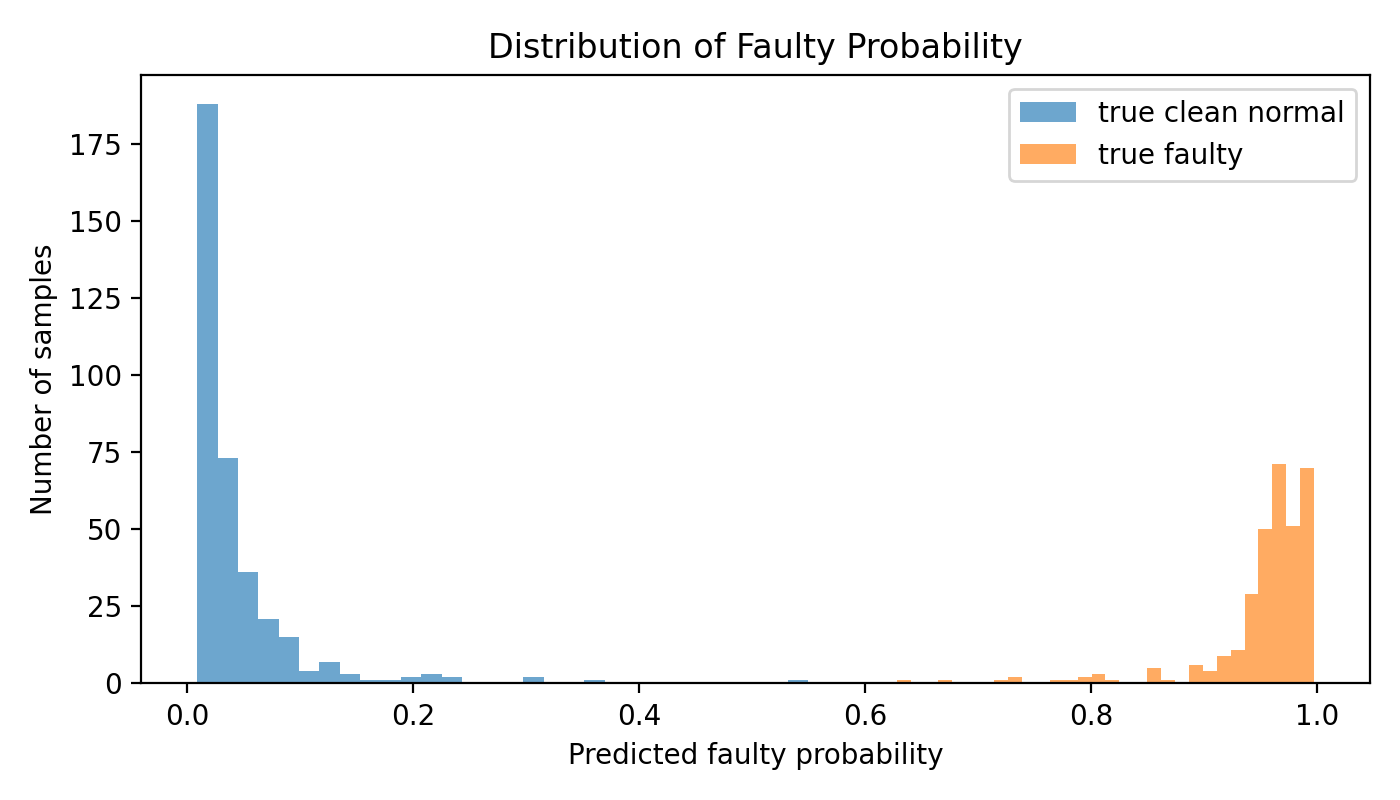
\includegraphics[width=0.85\linewidth]{05_faulty_probability_distribution.png}
    \caption{模型输出的 faulty probability 分布。真实 normal 样本主要接近 0，真实 faulty 样本主要接近 1，说明两类样本在指标事件日志上具有明显可分性。}
\end{figure}

\subsection{异常特征重要性}

\begin{figure}[H]
    \centering
    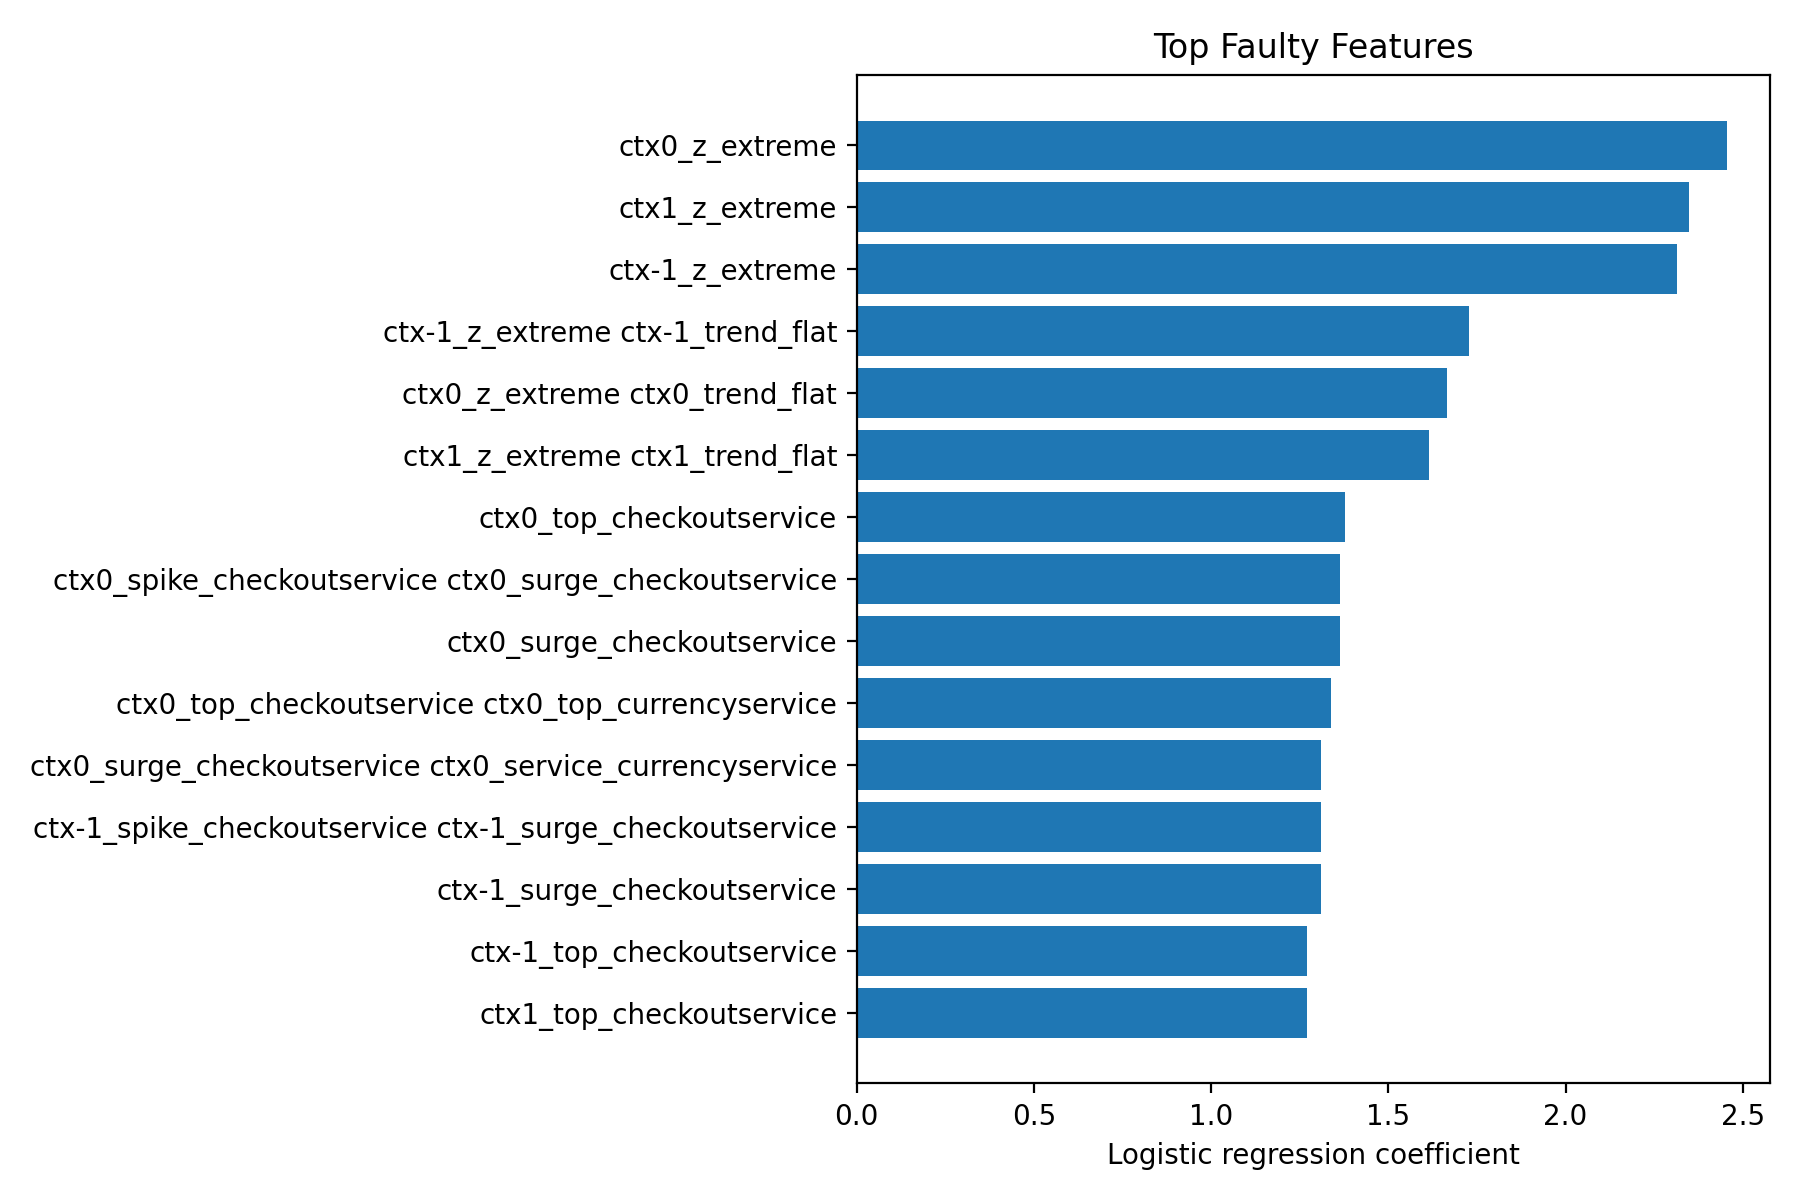
\includegraphics[width=0.90\linewidth]{06_top_faulty_features.png}
    \caption{Top faulty features。模型主要依据 z\_extreme、spike\_checkoutservice、surge\_checkoutservice 等特征判断异常，与 checkoutservice CPU 过载等故障现象一致。}
\end{figure}

\section{AIOps Agent 封装}

\subsection{Agent 设计目标}

根据作业要求，成员 F 需要实现一个 Python Agent，其逻辑包括：

\begin{enumerate}[label=\arabic*.]
    \item \textbf{触发器}：监听 Prometheus 告警或成员 E 的算法结果；
    \item \textbf{诊断逻辑}：调用大模型 API 或规则模块解释错误信息；
    \item \textbf{动作}：给出 Kubernetes 修复指令，例如 \texttt{kubectl delete pod} 或 \texttt{kubectl rollout restart}。
\end{enumerate}

综合实现难度和项目状态，本实验选择监听成员 E 的算法结果 CSV 作为触发器。原因是 Prometheus 告警监听需要额外配置 Alertmanager、告警规则和 Webhook，并依赖集群持续在线；而成员 E 的算法结果 CSV 可以离线运行，适合课程展示和稳定复现。

\subsection{Agent 输入格式}

Agent 监听的成员 E 检测结果格式如下：

\begin{lstlisting}[language=csv]
timestamp,anomaly_score,threshold,prediction,target_service,fault_type,evidence
2026-06-13 16:36:30,40156.73,61.5777,1,checkoutservice,cpu_pressure,
"cpu_checkoutservice mean robust z-score=167.3; z_extreme; spike_checkoutservice; surge_checkoutservice"
\end{lstlisting}

其中：

\begin{itemize}
    \item \texttt{prediction=1} 表示触发异常；
    \item \texttt{target\_service} 表示异常服务；
    \item \texttt{fault\_type} 表示故障类型；
    \item \texttt{evidence} 表示异常证据。
\end{itemize}

\subsection{Agent 运行方式}

Agent 默认以 dry-run 模式运行，只输出修复建议，不真正执行命令：

\begin{lstlisting}[language=bash]
python aiops_agent.py \
  --source member-e-csv \
  --input sample_member_e_detection_scores.csv \
  --namespace online-boutique \
  --max-events 3
\end{lstlisting}

若后续接入成员 E 的真实结果，只需将输入文件替换为：

\begin{lstlisting}[language=bash]
python aiops_agent.py \
  --source member-e-csv \
  --input detection_scores.csv \
  --namespace online-boutique \
  --max-events 5
\end{lstlisting}

\subsection{Agent 输出示例}

当 Agent 检测到 checkoutservice CPU 压力异常时，会输出：

\begin{lstlisting}
Detected 3 anomaly event(s).

Event #1
 target_service: checkoutservice
 fault_type: cpu_pressure
 anomaly_score: 40156.73

[Diagnosis]
Root cause: checkoutservice CPU pressure / resource saturation

Safe first steps:
- 查看 pod CPU 使用率和最近事件，确认是否存在 CPU 尖峰；
- 如果服务持续无响应，可以重启对应 deployment；
- 后续优化建议：提高 CPU limit/request，或减少压测并发。

[DRY-RUN] Suggested commands:
kubectl get pods -n online-boutique | grep checkoutservice
kubectl describe pod -n online-boutique -l app=checkoutservice
kubectl logs -n online-boutique -l app=checkoutservice --tail=100
kubectl top pod -n online-boutique | grep checkoutservice
kubectl rollout restart deployment/checkoutservice -n online-boutique
\end{lstlisting}

\begin{figure}[H]
    \centering
    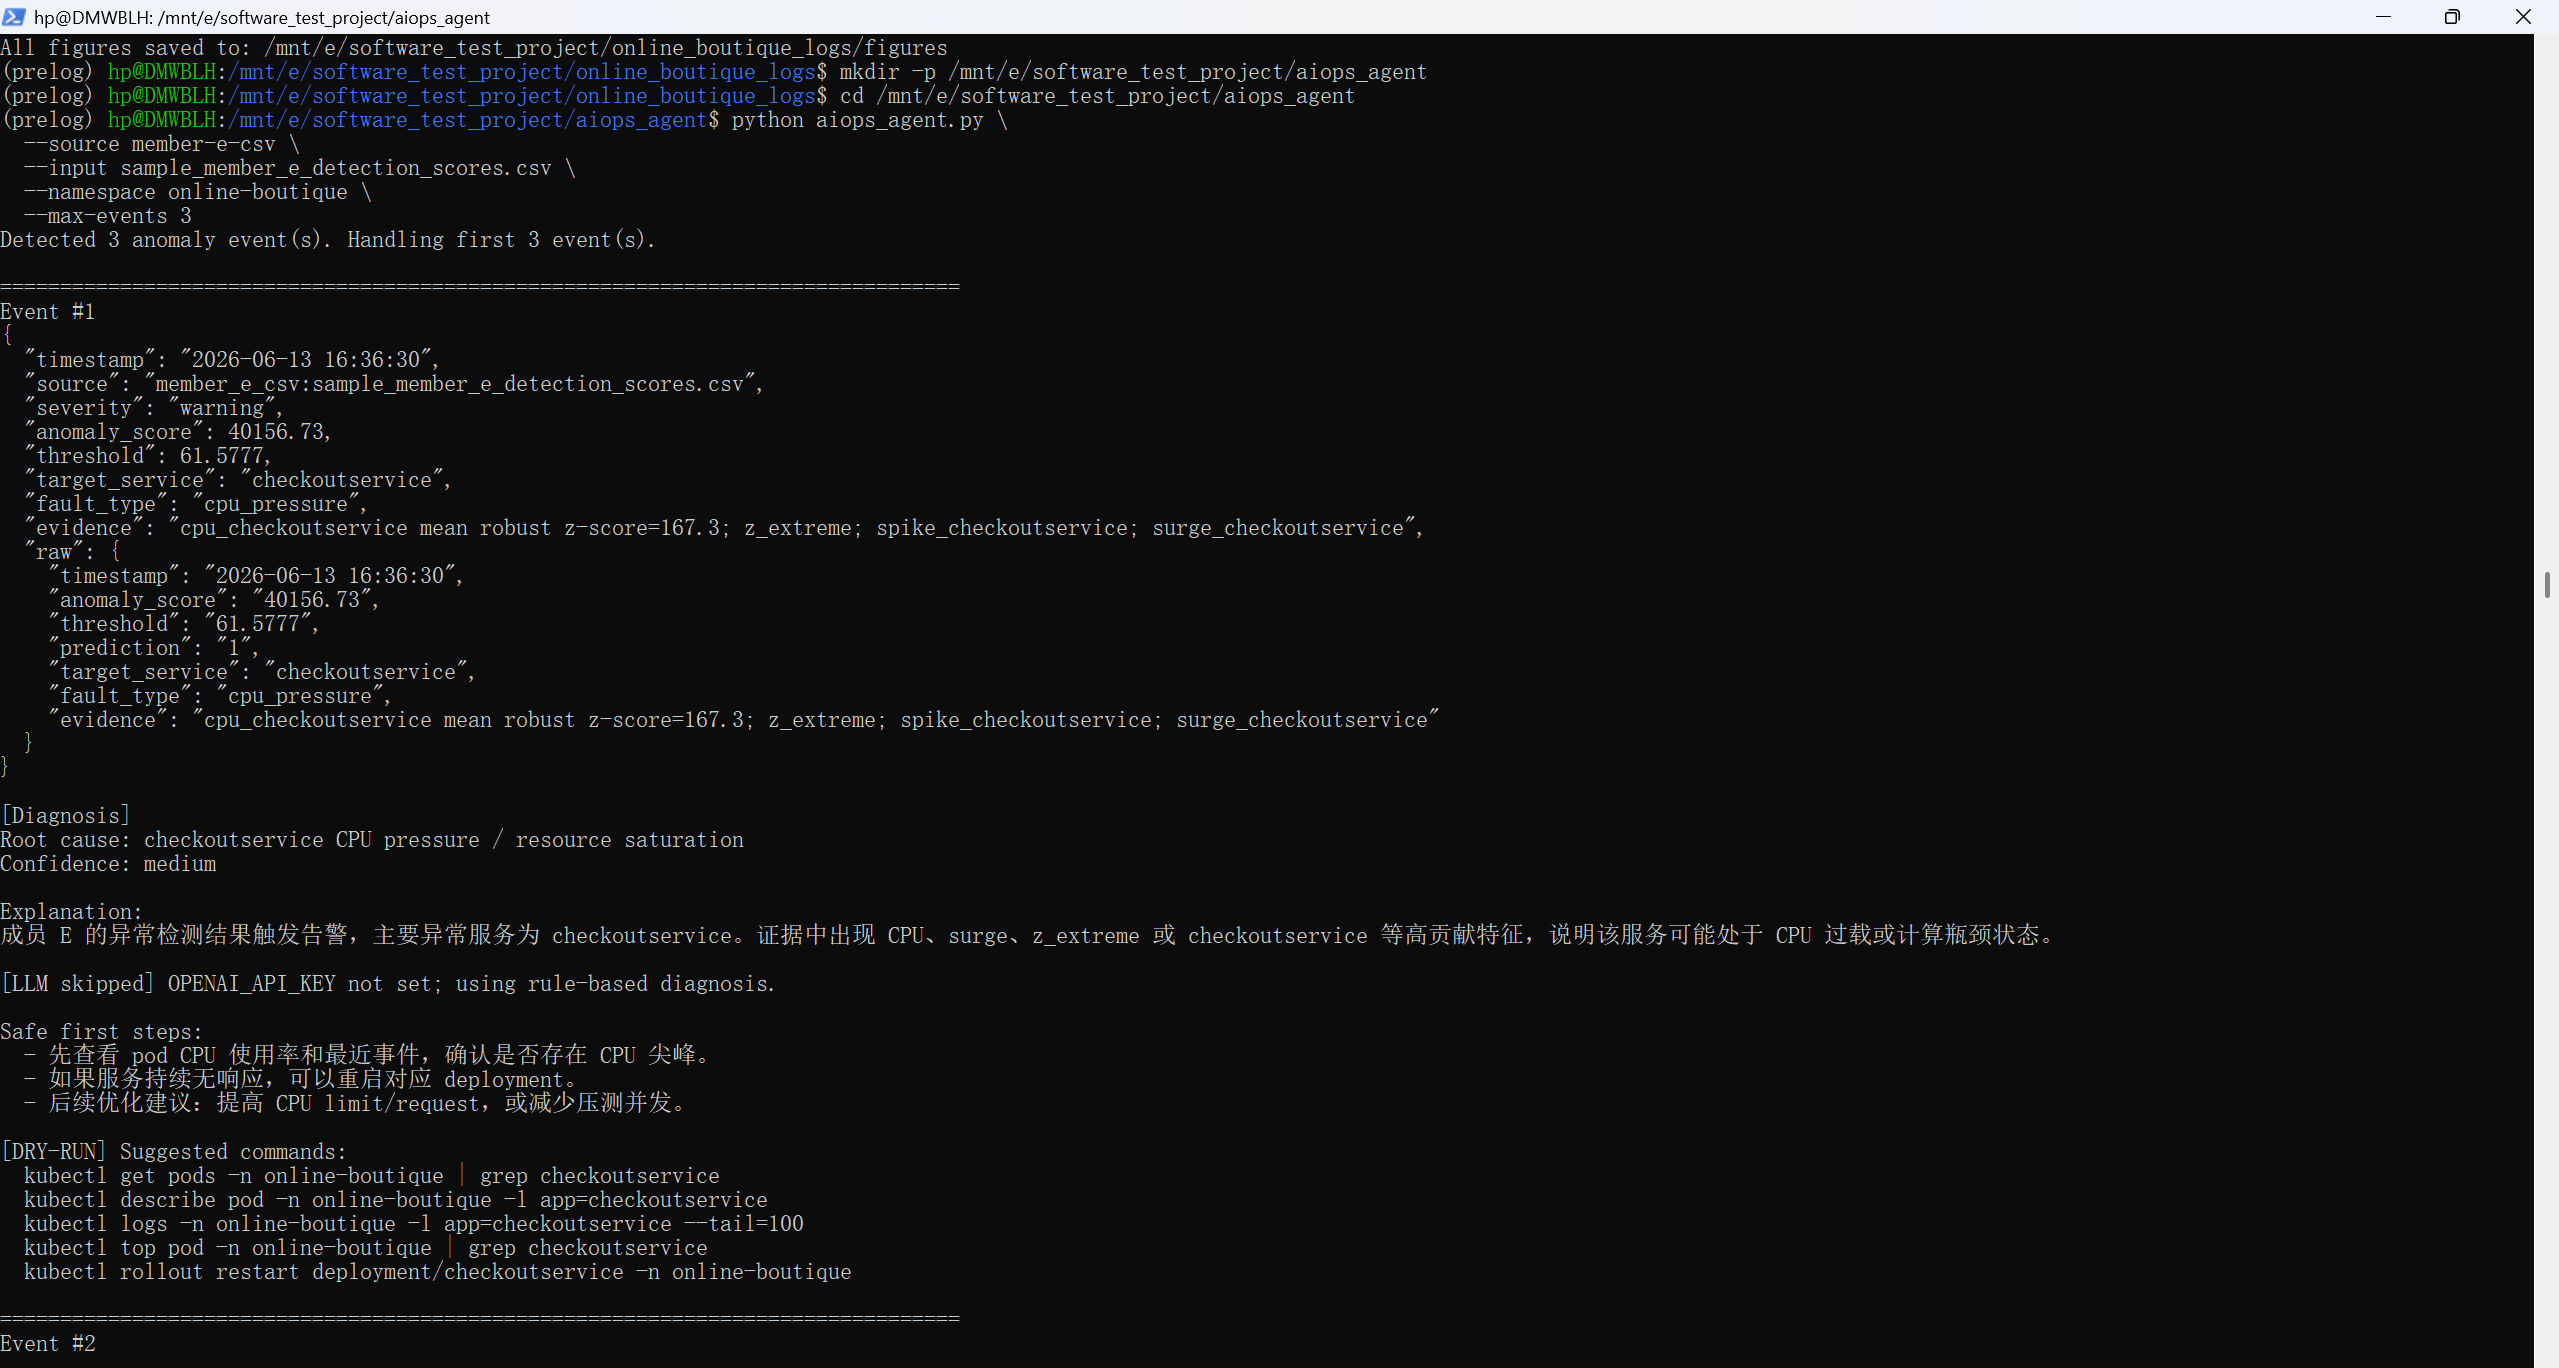
\includegraphics[width=0.95\linewidth]{Agent_demo_screenshot.png}
    \caption{AIOps Agent mock 演示截图。Agent 完成异常触发、根因解释和 kubectl 修复建议生成。}
\end{figure}

\subsection{三类故障对应动作}

\begin{center}
\begin{tabular}{p{3cm}p{4cm}p{6cm}}
\toprule
故障类型 & 目标服务 & Agent 输出动作 \\
\midrule
CPU 过载 & checkoutservice & \texttt{kubectl top pod}，查看日志，重启 deployment \\
网络延迟 & frontend & 检查 NetworkChaos、service endpoint，必要时重启 frontend \\
Pod Kill & cartservice & 查看 Kubernetes events，删除异常 Pod 让 deployment 自动拉起 \\
\bottomrule
\end{tabular}
\end{center}

\subsection{是否调用大模型 API}

Agent 代码中已预留 OpenAI-compatible API 调用接口。如果设置 \texttt{OPENAI\_API\_KEY}，Agent 会把异常事件和初步规则诊断发送给大模型生成自然语言解释；如果没有 API key，则自动退化为规则诊断，保证离线环境也能运行。

\begin{lstlisting}[language=bash]
export OPENAI_API_KEY="your_api_key"
export OPENAI_MODEL="gpt-4o-mini"
\end{lstlisting}

当前实验展示使用 mock 数据和规则诊断完成端到端验证。

\section{综合结论}

本成员完成的工作可以总结为以下几点：

\begin{enumerate}[label=\arabic*.]
    \item \textbf{PreLog 论文复现成功}：在官方 BGL 数据集上跑通 PreLog 流程，异常类 \texttt{faulty} F1-score 达到 0.935；
    \item \textbf{Online-Boutique 迁移存在退化}：直接迁移 PreLog 到本组数据时出现单类别退化，说明 PreLog 对小规模微服务业务日志和指标事件日志的迁移能力有限；
    \item \textbf{组内指标数据具有有效异常信号}：Metric-Event Baseline 在测试集上达到 accuracy 0.9985、macro F1 0.9985、faulty F1 0.9984，说明 Prometheus 指标事件日志具备明显可分性；
    \item \textbf{完成 AIOps Agent 封装}：Agent 能监听成员 E 的异常检测结果，生成根因解释和 kubectl 修复建议，形成检测、诊断、处置闭环。
\end{enumerate}

最终建议在汇报中采用如下叙述逻辑：

\begin{quote}
成员 F 首先完成 PreLog 论文复现，并在官方 BGL 数据集上得到较好结果。随后将 PreLog 迁移到 Online-Boutique 组内数据时发现单类别退化，说明论文模型在小规模微服务数据上存在迁移局限。为验证数据本身有效性，进一步构造 Metric-Event 日志并训练传统文本分类 baseline，证明指标事件中确实存在明显故障信号。最后封装 AIOps Agent，将成员 E 的异常检测结果转化为根因解释和 kubectl 修复建议，形成智能运维闭环。
\end{quote}

\section{PPT 素材建议}

若将本报告交给 AI 或组员生成 PPT，建议按以下页面组织：

\begin{enumerate}[label=\arabic*.]
    \item 成员 F 工作概览：PreLog 复现、Online-Boutique 迁移、baseline 验证、Agent 封装；
    \item PreLog 方法简介与 BGL 复现结果；
    \item Online-Boutique 数据构造与故障时间线；
    \item PreLog 迁移失败/单类别退化分析；
    \item Metric-Event Baseline 结果：混淆矩阵、概率分布、Top faulty features；
    \item AIOps Agent：触发器、诊断逻辑、动作模块；
    \item 总结：复现成功、迁移局限、数据验证、智能运维闭环。
\end{enumerate}

\end{document}
